\documentclass{article}
\usepackage{amsmath}
\usepackage{graphicx}
\usepackage{geometry}
\usepackage{amsfonts}
\usepackage{amssymb}
\usepackage{graphicx}
\usepackage[utf8]{inputenc} %Spanish input                                      
\usepackage[T1]{fontenc} % Use 8-bit encoding that has 256 glyphs 
\usepackage[spanish, es-tabla]{babel}        
\usepackage{float}
\usepackage{lscape}
\usepackage{enumerate}
\usepackage{color}
\usepackage{algpseudocode}
\usepackage{mathtools}
\usepackage{wrapfig}
\usepackage{subfig}
\usepackage{cite} % para contraer referencias
\usepackage[hidelinks]{hyperref}
\usepackage{xstring}
\usepackage{listings}
\usepackage{lipsum}
\usepackage{courier}
\usepackage{fancyhdr}
\usepackage[ruled,vlined,linesnumbered]{algorithm2e}
\usepackage{setspace}


%------------------------------------------------------------------------
\newtheorem{theorem}{Theorem}
\newtheorem{acknowledgement}[theorem]{Acknowledgement}
%\newtheorem{algorithm}[theorem]{Algorithm}
\newtheorem{axiom}[theorem]{Axiom}
\newtheorem{case}[theorem]{Case}
\newtheorem{claim}[theorem]{Claim}
\newtheorem{conclusion}[theorem]{Conclusion}
\newtheorem{condition}[theorem]{Condition}
\newtheorem{conjecture}[theorem]{Conjecture}
\newtheorem{corollary}[theorem]{Corollary}
\newtheorem{criterion}[theorem]{Criterion}
\newtheorem{definition}[theorem]{Definition}
\newtheorem{example}[theorem]{Example}
\newtheorem{exercise}[theorem]{Exercise}
\newtheorem{lemma}[theorem]{Lemma}
\newtheorem{notation}[theorem]{Notation}
\newtheorem{problem}[theorem]{Problem}
\newtheorem{proposition}[theorem]{Proposition}
\newtheorem{remark}[theorem]{Remark}
\newtheorem{solution}[theorem]{Solution}
\newtheorem{summary}[theorem]{Summary}
\newenvironment{proof}[1][Proof]{\textbf{#1.} }{\ \rule{0.5em}{0.5em}}
\pagestyle{fancy}
\setlength{\textwidth}{7.0in}
\setlength{\oddsidemargin}{-0.35in}
\setlength{\topmargin}{-0.5in}
\setlength{\textheight}{9.0in}
\setlength{\parindent}{0.3in}
\setlength{\pdfpagewidth}{88.184mm}
\setlength{\pdfpageheight}{113.854mm}
\setlength{\footskip}{12.0pt}


\newcommand{\thelink}{\@empty}
\newcommand{\link}[2]{%
  \IfSubStr{#1}{:}{\renewcommand\thelink{#1}}{\renewcommand\thelink{#1:#2}}%
  \href{\thelink}{\texttt{#2}}%
}
%--------------------------------------------------------------
\geometry{
  a4paper,
  left=30mm,
  right=30mm,
  headheight=3cm,
  top=2.5cm,
  bottom=3.5cm,
  footskip=0cm
}
\begin{document}[\scriptsize]
\begin{titlepage}
\title{METAHEURISTICAS PRACTICA 1}
\author{Pablo Huertas Arroyo}
\date{ \today }


\maketitle
\begin{figure}[h]
    \centering
    
\includegraphics[scale=4]{LogoUGR.png}
\end{figure}


\hspace{-1.7cm}
\newline Correo: \link{mailto}{phuertas@correo.ugr.es}
\newline DNI:77033078Y
\newline Grupo 3A, subgrupo 2
\newline Horario: Lunes de 17:30 a 19:30
\end{titlepage}

\newpage
\tableofcontents


\newpage
\section{\large INTRODUCCION AL PROBLEMA ABORDADO}
\large El problema elegido a abordar en esta practica es el siguiente:
Problema de la mínima dispersión diferencial\textbf{(MDD)}.
Es un problema de optimización combinatoria consistente en
seleccionar un subconjunto M de m elementos (|M|=m) de un conjunto inicial N de n
elementos (con n>m) de forma que se minimice la dispersión entre los elementos
escogidos.

Este problema tiene diferentes \textbf{aplicaciones en el campo de la optimización},
como pueden ser la elección de la localización de elementos públicos, selección
de grupos homogéneos, identificación de redes densas, reparto equitativo, problemas
de flujo, etc

\begin{figure}[h]
    \centering
    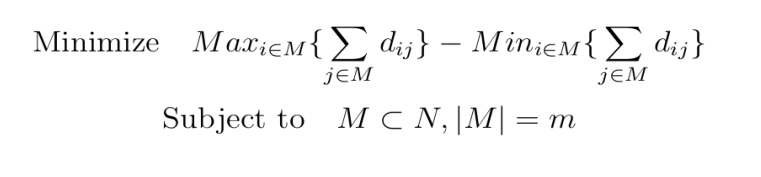
\includegraphics[scale=0.5]{FormulaMinimizacion.png}
\end{figure}

donde:
\begin{itemize}
\item M es una solución al problema que consiste en un vector binario que indica los m
elementos seleccionados
\item$d_{ij}$ es la distancia existente entre los elementos i y j.
\end{itemize}

Para resolver este problema se utilizarán 50 casos seleccionados con distancias reales
con, n entre {25,50,75,100,125,150}, y m enttre 2 y 45.

\vspace{5mm} 

La Dispersión de una Solución es la diferencia de los valores extremos, es decir,
la diferencia de la sumas de las distancias de dichos puntos al resto de los puntos.
Por ejemplo, si tenemos 8 puntos para colocar farmacias, y solo podemos colocar 4,
\textbf{¿cuál es la forma de colocarlas, de forma que se reduzca la dispersión?}

\vspace{5mm}

Esto es lo que realizamos en esta prácticas, donde probaremos diferentes algoritmos
para resolver el problema, y los compararemos entre ellos para poder extraer nuestras
propias conclusiones.

\newpage

\section{\large ESQUEMA COMÚN}

\subsection{\large Representación de soluciones}
Para esta práctica, he implementado 7 algoritmos distintos.

\begin{itemize}
\item Algoritmo 1: \textbf{Algoritmo Genético Generacional con cruce Uniforme}
\item Algoritmo 2: \textbf{Algoritmo Genético Generacional con cruce de Posición}
\item Algoritmo 3: \textbf{Algoritmo Genético Estacionario con cruce Uniforme}
\item Algoritmo 4: \textbf{Algoritmo Genético Estacionario con cruce de Posición}
\item Algoritmo 5: \textbf{Algoritmo Memético con 3 variantes diferentes}
\begin{itemize}
\item Algoritmo 5.1: \textbf{AM con BL en todos los cromosomas}
\item Algoritmo 5.2: \textbf{AM con BL en los N*0'1 mejores cromosomas}
\item Algoritmo 5.3: \textbf{AM con BL en N*0'1 aleatorios cromosomas}
\end{itemize}

\end{itemize}

\vspace{5mm}

Los datos se encuentran en unos ficheros \emph{.txt}, donde hay una primera línea 
que indica el numero de elementos \emph{n} y el número de elementos a seleccionar
\emph{m} del problema.
\newline Luego se encuentran \textbf{\emph{n*(n-1)/2}} líneas con el formato i,j,$d_{ij}$ que
tienen el contenido de las \textbf{distancias entre los elementos}.
\newline En mi caso, para los dos algoritmos he leido estos ficheros
y he almacenado los datos en una matriz distancias completa, donde la diagonal es 0,
y las triangulares superiores e inferiores son simétricas entre sí.

\vspace{5mm}

La posición (2,3) de la matriz distancias es la distancia entre los elementos 2 y 3,
que a su vez es la misma que la posición (3,2).

\vspace{5mm}

La \textbf{representación de la solución} es un vector binario, donde la posición i-ésima
es 1 si el elemento i-ésimo está seleccionado, y 0 en caso contrario.

\vspace{5mm}

Para la \textbf{factorización de la función objetivo}, a la hora de generar una nueva solución no
es necesario volver a calcular por completo el vector de distancias para obtener la nueva
dispersión. Basta con restar la distancia a cada elemento de la solución al elemento que 
se ha quitado de la solución actual, y sumarle la distancia del nuevo elemento a todas las demás 
de la solución.
\newline Entonces,teniendo el vector de distancias actualizado, para saber la dispersión de dicho conjunto 
de elementos restamos la mayor distancia de dicho vector con la menor

\vspace{5mm}

Debido a que se requiere aleatoriedad en ambos algoritmos, ya que son probabilísticos, he usado un vector de semillas, 
donde en cada iteración que 
realiza cada algoritmo se genera una nueva semilla, y se utiliza para generar nuevas soluciones.
El valor estático de la semilla sirve para que cada vez que se ejecute el algoritmo, se obtengan las mismas Soluciónes.

También se pedía calcular el tiempo de ejecución de cada algoritmo, por lo que he usado objetos de la clase 
\textbf{<chrono>} para tener una alta precisión en los tiempos, y los muestro en \textbf{segundos}.

\vspace{5mm}

Al finalizar cada algoritmo calculo el tiempo demorado por dicho algoritmo y la dispersión de la 
mejor solución de la población.

\subsection{\large Descripción de la función objetivo}
La función objetivo de este problema es la de encontrar la dispersión a partir de un vector de 
booleanos donde la posición i-ésima es 1 si el elemento i-ésimo está seleccionado, y 0 en caso contrario.\\
Para evaluar la función objetivo, se convierte internamente el vector de booleanos en una selección 
de elementos de números enteros.\\
Para ello, se recorre el vector de booleanos, y si la posición i-ésima es 1, se añade al final del vector de 
seleccionados el elemento i-ésimo.\\
Tenemos la matriz de distancias comentada anteriormente, y la selección de elementos, por lo
que para evaluar la función objetivo, para cada elemento del vector de seleccionado, en la posición i-ésima
del vector distancias, añadimos la distancia del elemento i-ésimo a todos los demás elementos del vector de seleccionados.\\
Las posiciones se corresponden 1 a 1 en los vectores de seleccionados y distancias.
\vspace{5mm}

\begin{algorithm}
  \scriptsize
  \label{Algoritmo de Evaluacion de la Funcion Objetivo}
  \caption{Algoritmo de Evaluación de la Función Objetivo}
  \KwIn{distancias(vector), seleccionados(vector), m(matriz distancias)}% Parámetros de entrada
  $distancias \leftarrow 0$\\
  
\vspace{3mm}

\vspace{3mm}
$Vector Distancias \leftarrow{\emph{GenerarVectorDistancias()}}$\\
$Dispersion Comparacion \leftarrow{\emph{Calculardispersion(VectorDistancias)}}$\\
\vspace{3mm}
$Mejora \leftarrow {\textbf{TRUE}}$\\

\For{$i \in Size(seleccionados)$}{
  $a comparar \leftarrow i $\\
  \For{$j \in Size(seleccionados)$}{
    \If{$seleccionados[i] \neq acomparar$}{
      $distancias[i] += m[acomparar][seleccionados[i]]$\\
    }
  }
}
\end{algorithm}

\subsection{\normalsize Descripción de los operadores comunes}
Hay ciertos operadores y funciones que son comunes para los algoritmos desarrollados en esta práctica,
ya que por ejemplo la generación de soluciones aleatorias para la población inicial es común y varios operadores 
más, por lo que voy a desglosar uno a uno para entrar más en profundidad.

\subsubsection{\small Operador de generación de vecino}

\vspace{3mm}

\subsubsection{\small Generación de soluciones aleatorias}
Para la generación de la primera población aleatoria, utilizo dos funciones distintas, una para generar soluciones 
aleatorias, y otra que genera una población completa de tamaño $50$, donde $50$ es el tamaño de la población que vamos a usar en todos los algoritmos.\\
La segunda función es la que llama a la primera $50$ veces.
\begin{algorithm}
  \label{Algoritmo de Generacion de Soluciones Aleatorias}
  \caption{Algoritmo de Generación de Soluciones Aleatorias}
  \KwIn{n(número de puntos) m(número de puntos a seleccionar), semilla(número que simboliza una semilla estática) }% Parámetros de entrada
  \KwOut{solucion(vector de booleanos)}% Parámetros de salida
\vspace{3mm}

$solucion \leftarrow \emptyset $\\
$seleccionados \leftarrow \emptyset $\\
\vspace{3mm}

\While{$Size(seleccionados) < m$}{
  $seleccionados \leftarrow \emph{Numero aleatorio que no esta en seleccionados} $\\
  $solucion \leftarrow \emph{seleccionados.back} $\\
}
\end{algorithm}

\begin{algorithm}[H]
  \scriptsize
  \label{Algoritmo de Generacion de Poblaciones Aleatorias}
  \caption{Algoritmo de Generación de Poblaciones Aleatorias}
  \KwIn{n(número de puntos) m(número de puntos a seleccionar), semilla(número que simboliza una semilla estática), matrizdatos(matriz distancias) }% Parámetros de entrada
  \KwOut{p(poblacion generada)}% Parámetros de salida
\vspace{3mm}

$p \leftarrow \emptyset $\\
\vspace{3mm}

\For{$i \in 50 $}{
  $solucion \leftarrow \emph{GeneraSolucionAleatoria(n,m)} $\\
  $seleccionados \leftarrow \emptyset $\\
  \For{$j \in Size(solucion)$}{
    \If{ ($solucion[j] != 0)$}{
      $seleccionados \leftarrow \emph{j}$
    }
  }
  $Algorithm1--> Evaluacion de la Funcion Objetivo $\\
  $p \leftarrow \emph{solucion} $\\
  
}
\end{algorithm}

\subsubsection{\small Mecanismo de selección en los Algoritmos Genéticos}
Para estos algoritmos, en el mecanismo de selección hemos usado el torneo binario, que 
consiste en elegir dos individuos aleatorios de la población y seleccionar el que 
mejor fitness, en este caso menor dispersión, de estos.
En el esquema generacional, se aplican $n$ torneos binarios, donde $n$ es el tamaño de la población.
En cambio en el esquema estacionario, se aplican solamente 2 torneos binarios, que darán lugar a los dos
padres que posteriormente son cruzados.

\begin{algorithm}[H]
  \scriptsize
  \label{Algoritmo de Seleccion}
  \caption{Algoritmo de Selección}
  \KwIn{p(poblacion)}% Parámetros de entrada
  \KwOut{pnueva(poblacion generada)}% Parámetros de salida
\vspace{3mm}

$pnueva \leftarrow \emptyset $\\
\eIf{$emph{Esquema Generacional}$}
{
  $numero$ $iteraciones \leftarrow \emph{n}$\\  
}{
  $numero$ $iteraciones \leftarrow \emph{2}$\\
}
\vspace{3mm}

\For{$i \in numero iteraciones $}{
  $posicion1 \leftarrow \emph{GenerarNumeroAleatorioEntre(0, n)} $\\
  $posicion2 \leftarrow \emph{GenerarNumeroAleatorioEntre(0, n)} $\\
  $\emph{Las posiciones no deben ser iguales}$ \\

  \eIf{$dipersion(posicion1) < dipersion(posicion2)$}
  {
    $pnueva \leftarrow \emph{p(posicion1)} $\\
  }{
    $pnueva \leftarrow \emph{p(posicion2)} $\\
  }
}
$return$ $pnueva $\\
\end{algorithm}


\subsubsection{\small Operadores de cruce}
Para estos algoritmos, he usado dos operadores de cruce distintos.
En el primero a partir de dos padres se generan dos hijos, mientras que en 
el segundo se genera un solo hijo.
Ambos tienen en común que las posiciones que contienen el mismo valor en ambos padres se mantienen 
en los dos hijos generados.

\begin{itemize}
\item Cruce de Posición\\
Las posiciones (genes) restantes de ambos padres se desordenan aleatoriamente de forma independiente, y se completan 
los huecos en ambos hijos con dichos valores desordenados. \\
Por lo tanto, esto da lugar a dos soluciones válidas (con m 1's) que en este caso 
son los hijos 

\begin{algorithm}[H]
  \scriptsize
  \label{Operador de Cruce Basado en Posicion}
  \caption{Operador de Cruce Basado en Posición}
  \KwIn{ p1(padre 1), p2(padre2) }% Parámetros de entrada
  \KwOut{ h1(hijo1), h2(hijo2) }% Parámetros de salida
\vspace{3mm}

$restantesp1 \leftarrow \emptyset $\\
$restantesp2 \leftarrow \emptyset $\\
$posiciones$ $no$ $asignadas \leftarrow \emptyset $\\
\vspace{3mm}
\For{$i \in n $}{
  \eIf{$ Disintos( p1[i], p2[i] )  $}
  {
    $\emph{Si el gen en la posicion i es distinto en ambos padres,
    no lo heredan}$\\
    $restantesp1 \leftarrow \emph{p1[i]} $\\
    $restantesp2 \leftarrow \emph{p2[i]} $\\
    $posiciones$ $no$ $asignadas \leftarrow \emph{i} $\\
  }{
    $\emph{Si el gen en la posicion i es igual en ambos padres,
    lo heredan}$\\
    $h1[i] \leftarrow \emph{p1[i]} $\\
    $h2[i] \leftarrow \emph{p2[i]} $\\
  }  
}
$restantesp1 \leftarrow \emph{Desordenar aleatoriamente} $\\
$restantesp2 \leftarrow \emph{Desordenar aleatoriamente} $\\

\vspace{3mm}
\For{$i \in Size(restantesp1) $}{
  $h1[posiciones$ $no$ $asignadas[i]] \leftarrow \emph{restantesp1[i]} $\\
  $h2[posiciones$ $no$ $asignadas[i]] \leftarrow \emph{restantesp2[i]} $\\
}
\vspace{3mm}
$return h1,h2 $\\

\end{algorithm}

\vspace{3mm}
\item Cruce Uniforme \\
Las selecciones restantes se seleccionan aleatoriamente de un padre o de otro, lo que puede dar
lugar a un hijo cuya solución no sea válida.\\
Por lo tanto, necesitamos un operador de reparación, que lo que hace es dada una solución con 
x 1's, la convierte en una solución con m 1's, para que sea válida.

\begin{algorithm}[H]
  \scriptsize
  \label{Operador de Cruce Basado en Posicion}
  \caption{Operador de Cruce Basado en Posición}
  \KwIn{ p1(padre 1), p2(padre2) }% Parámetros de entrada
  \KwOut{ h(hijo) }% Parámetros de salida
\vspace{3mm}


$posiciones$ $no$ $asignadas \leftarrow \emptyset $\\
\For{$i \in n $}{
  \eIf{$ Disintos( p1[i], p2[i] )  $}
  {
    $posiciones$ $no$ $asignadas \leftarrow \emph{i} $\\
    \eIf{$GenerarNumeroAleatorioEntre(0,1) == 0 $}{
      $h[i] \leftarrow \emph{p1[i]} $\\
    }{
      $h[i] \leftarrow \emph{p2[i]} $\\
    }
  }{
    $\emph{Si el gen en la posicion i es igual en ambos padres,
    lo heredan}$\\
    $h[i] \leftarrow \emph{p1[i]} $\\
  }  
}
$numero$ $de$ $escogidos \leftarrow \emph{ContarSeleccionadosEn(h)} $\\
\vspace{3mm}

\If{$numero$ $de$ $escogidos != m$}{
  $h \leftarrow \emph{Reparar(h)} $\\
}

$return$ $h $\\

\end{algorithm}



\begin{algorithm}[H]
  \scriptsize
  \label{Operador de Reparacion}
  \caption{Operador de Reparación}
  \KwIn{ h(hijo), v(pos a rellenar) }% Parámetros de entrada
  \KwOut{ h(ijo) }% Parámetros de salida
\vspace{3mm}


$cantidad$ $a$ $reparar  \leftarrow m - \emph{ContarSeleccionadosEn(h)} $\\
$distancias \leftarrow GenerarDistancias(h) $\\
$mediadistancias \leftarrow Media(distancias) $\\
\vspace{3mm}
\eIf{$cantidad$ $a$ $reparar < 0$}{
  $\emph{Sobran elementos seleccionados}$\\
  \While{$cantidad$ $a$ $reparar < 0$}{
    $\emph{Busco el elemento cuyas distancias se alejen mas de la media}$\\
    $posicion \leftarrow 0 $\\
    $distanciamayor \leftarrow 0 $\\
    \For{$i \in Size(distancias) $}{
      \If{$ ABS(distancias[i]-mediadistancias) > distanciamayor $}{
        $distanciamayor \leftarrow ABS(distancias[i]-mediadistancias) $\\
        $posicion \leftarrow i $\\
      }
    }

    $\emph{Elimino dicho elemento seleccionado de la solucion del hijo}$\\
    $h[posicion] \leftarrow \emph{v} $\\
    $cantidad$ $a$ $reparar \leftarrow cantidad$ $a$ $reparar + 1 $\\
  }
}{
  $\emph{Faltan elementos seleccionados}$\\
  \While{$cantidad$ $a$ $reparar > 0$}{
    $\emph{Busco el elemento que minimice la media de distancias}$\\
    $posicion \leftarrow 0 $\\
    $mediamin \leftarrow 0 $\\
    \For{$i \in Size(h) $}{
      $\emph{Pruebo uno a uno añadiendo los elementos no seleccionados a la solucion}$\\
      \If{$media con nuevo elemento < mediamin $}{
        $mediamin \leftarrow media $\\
        $posicion \leftarrow i $\\
      }
    }
  }


  $\emph{Añado dicho elemento no seleccionado de la solucion del hijo}$\\
  $h[posicion] \leftarrow \emph{v} $\\
  $cantidad$ $a$ $reparar \leftarrow cantidad$ $a$ $reparar - 1 $\\
}


$return$ $h $\\

\end{algorithm}


\end{itemize}
\subsubsection{\small Operador de mutación}
La mutacion consiste en modificar con cierta probabilidad uno o varios genes de la poblacion 
aleatoriamente. La probabilidad de mutacion es dada por la constante \emph{probabilidad 0.1}.
Cuando muta un gen de un cromosoma, tenemos que encontrar otro gen del mismo cromosoma con el valor contrario,
para mantener la factibilidad de la solucion de dicho cromosoma.
Por ejemplo, en una solucion con 10 elementos donde se seleccionan 3, si se va a mutar el segundo seleccionado, tenemos que buscar uno de los 7
elementos que no esten seleccionados de manera aleatoria y cambiar el valor de cada gen.
El rango de elementos que pueden ser mutados, van desde 0 hasta el producto del numero de cromosomas por el numero de genes 
por cromosoma.\\
Si la poblacion tiene 10 cromosomas, y cada cromosoma 5 genes, si se genera para mutar el elemento 15, será el sexto gen del segundo cromosoma.

\begin{algorithm}[H]
  \scriptsize
  \label{Operador de Mutacion}
  \caption{Operador de Mutación}
  \KwIn{ p(poblacion), prob(probabilidad) }% Parámetros de entrada
  \KwOut{ pnueva(poblacion generada) }% Parámetros de salida
\vspace{3mm}

$rango$ $mutacion \leftarrow \emph{p.NumeroDeCromosomas()} \cdot \emph{p.NumeroDeGenesPorCromosoma()} $\\

\For{$i \in Size(p)$}{
  \If{$GenerarNumeroAleatorioEntre(0,1) < prob$}{
    $\emph{Genero aleatoriamente un elemento en el rango de mutacion}$\\
    $posicion \leftarrow GenerarNumeroAleatorioEntre(0,rango) $\\

    $\emph{Para el elemento de la posicion generada, busco otro gen del mismo cromosoma 
    con el valor contrario}$\\
    $posicion2 \leftarrow \emph{Gen del mismo cromosoma aleatorio con valor contrario} $\\

    $\emph{Swap(posicion, posicion2)}$\\
  }

}
$return$ $pnueva$\\ 

\end{algorithm}

\newpage
\section{\large ESTRUCTURA DE MÉTODO DE BÚSQUEDA}

\subsection{\normalsize Pseudocódigo del método de búsqueda}
La estructura general del método de búsqueda es la siguiente:
\begin{itemize}
\item Primero de aplica el operador de selección, de donde la poblacion actual se 
selecciona los que van a formar la poblacion siguiente.
\item Segundo, se aplica el operador de cruce, donde con cierto porcentaje dependiendo
del esquema de cruce escogido, se cruzan padres con los operadores vistos anteriormente 
para dar lugar a los nuevos hijos que van a formar la poblacion siguiente.
\item Tercero, se aplica el operador de mutación, donde con cierto porcentaje 
pueden mutar x genes, pero siempre las soluciones son factibles.\\
Es decir, si tiene que haber m elementos seleccionados y se elige mutar el segundo elemento del 
cromosoma y, se ha de encontrar otro gen que tenga el valor contrario al mutado, para que cambie tambien
su valor y la solucion siga siendo factible
\item Como cuarto y ultimo, se aplica el operador de reemplazamiento, donde dependiendo del
esquema que se haya usado, se realiza de una forma u otra. Es la última fase que va a dar
lugar a la población completa que va a sustituir a la que había en el momento del 
inicio de la seleccion.\\
En el esquema generacional, solo se comprueba si en la poblacion 
nueva se ha perdido la mejor solucion que habia en la poblacion actual, y si es así, se
sustituye por la peor solucion en la poblacion nueva. Esto se hace para conservar las 
mejores soluciones que van apareciendo en la ejecucion del algoritmo. Este proceso se llama elitismo.\\
En el esquema estacionario, la nueva poblacion solo tiene 2 cromosomas, y estas dos soluciones 
compiten por entrar en la poblacion contra las dos peores de estas. 

\end{itemize}

\begin{algorithm}[H]
  \scriptsize
  \label{Estrctura del Metodo de búuqueda}
  \caption{Estrctura del Método de búsqueda}
  \KwIn{p(poblacion)}% Parámetros de entrada
  \KwOut{pnueva(poblacion generada)}% Parámetros de salida
\vspace{3mm}
$num$ $evaluaciones \leftarrow 0 $\\
$pnueva \leftarrow p $\\
\While{$num$ $evaluaciones < 100000$}{
  $poblacionauxiliar \leftarrow p $\\
  $poblacionauxiliar \leftarrow OperadorSeleccion(poblacionauxiliar) $\\
  $poblacionauxiliar \leftarrow OperadorCruce(poblacionauxiliar) $\\
  $poblacionauxiliar \leftarrow OperadorMutacion(poblacionauxiliar) $\\
  $pnueva \leftarrow OperadorReemplazo(poblacionauxiliar) $\\ 
  $num$ $evaluaciones \leftarrow num$ $evaluaciones + \emph{veces que han sido calculadas las distancias de las soluciones} $\\ 
}

$return$ $pnueva $\\
\end{algorithm}

\subsection{\normalsize Algoritmos Genéticos y reemplazamiento}
\subsubsection{\small Esquema de evolución}
En esta práctica vemos dos esquemas distintos de evolución:
\begin{itemize}
\item Esquema generacional con elitismo. \\
Las poblaciones en cada iteracion nunca pierden la mejor solucion de esta
Por lo tanto, en el proceso de reemplazamiento se comprueba si se ha perdido la mejor
solucion de la poblacion t, y si es así, se sustituye por la peor solucion de la poblacion 
t+1, que es la que va a pasar a ser la actual en la proxima iteracion.\\
Con este esquema podemos ver que las poblaciones cambian de forma radical muy rapidamente.
\item Esquema estacionario. \\
Las poblaciones en cada iteración pueden como mucho perder las dos peores 
soluciones de esta, ya que entran en una especie de torneo donde compiten con las dos 
soluciones conseguidas en dicha iteracion. Las dos mejores serán las que se mantienen.
En este esquema, las poblaciones no cambian con tanta rapidez como el esquema generacional.
\end{itemize}

\subsection{\normalsize Algoritmos Meméticos}
Los algoritmos meméticos son técnicas de optimización que combinan conceptos 
tomados de otras metaheuristicas, como la búsqueda basadda en poblaciones y la busqueda 
de mejora local.
Estos algoritmos implementados, tienen la misma estructura que los algoritmos genéticos
generacionales, pero con la diferencia de que:
\begin{itemize}
\item En la primera variante del algoritmo, \emph{AM-(10,1.0)} Cada 10 generaciones, se aplica la BL sobre todos los
cromosomas de la población.
Es decir, cuando el numero de iteraciones es multiplo de 10, se aplica la BL sobre todos los
cromosomas de la población, lo que aumenta considerablemente la capacidad del 
algoritmo en buscar mejores soluciones.
\item En la segunda variante del algoritmo, \emph{AM-(10,0.1)} Cada 10 generaciones, se aplica la BL sobre un 
subconjunto de cromosomas de la población seleccionado aleatoriamente con probabilidad igual a 0.1 para cada cromosoma.
Es decir, cuando el numero de iteraciones es multiplo de 10, se aplica sobre n*0.1 aleatorios cromosomas de la 
poblacion la busqueda local.
\item En la tercera variante del algoritmo, \emph{AM-(10,0.1mej)} Cada 10 generaciones, se aplica la BL sobre los 10\%
mejores cromosomas de la poblacion. 
\end{itemize}

\subsubsection{\small Búsqueda Local(BL)}
 Este algoritmo es un tipo de algoritmos de busqueda por trayectorias simples.
\newline En este algoritmo, se empieza con una solución inicial completa y aleatoria,
es decir, una Solución con \emph{M} elementos que no se repiten entre sí.
El orden de estos elementos no es relevante.
\vspace{5mm}
%o Para el algoritmo BL, el métodos de exploración del entorno, el operador
%de generación de vecino, la factorización de la BL y la generación de
%Soluciónes aleatorias.
\newline La idea es tras haber generado una completa Solución aleatoria válida, generar el 
\textbf{vecindario completo} de la Solución actual, \textbf{desordenarlo aleatoriamente}, y recorrerlo 
comparando en cada iteracion si se mejora la Dispersión.
\newline Si se mejora la Dispersión, se \textbf{selecciona dicha Solución como Solución actual} y 
se vuelve a generar el vecindario. Este proceso se hace hasta que no se mejore la Dispersión con 
todo el vecindario generado o hasta que se hayan hecho \textbf{100000 evaluaciones de la funcion objetivo}.
Es decir, comprobar 100000 veces si se mejora la Dispersión.
\newline Como vemos este algoritmo se parece a Greedy en que ambos cuando encuentran una Solución 
mejor que la anterior la seleccionan, y no se espera en este caso a recorrer todo el vecindario para 
encontrar una mejor Solución. Es por eso que este algoritmo se llama Busqueda Local de \textbf{Primero el mejor}
\vspace{5mm}
\newline La generación de la primera Solución aleatoria se hace con un bucle que va generando 
numeros aleatorios entre 0 y n-1, de forma que si no se ha añadido aún a la Solución, lo añade.
Este proceso se repite hasta que el numero de elementos de la Solución sea igual a \emph{M}
\newline Para la generación de vecinos, uso un vector de tuplas, que contienen el elemento que se 
va a intercambiar y el elemento que se va a intercambiar y va a entrar a la Solución provisional.
\newline Por ejemplo, si tengo {M}=6 y {N}=3, Solución provisional=(1,3,5), y genero el vecindario de esta Solución, 
este será el vector de tuplas \newline {(1,0), (1,2) ,(1,4), (3,0), (3,2), (3,4), (5,0), (5,2), (5,4)}.
\newline Entonces, desordena este vector aleatoriamente y se va intercambiando la posicion primera 
de la tupla que se encuentra en la Solución por la segunda posicion de la tupla que no se encuentra en la Solución
\newline La factorización es la misma que en el algoritmo greedy, cuando se intercambia un elemento de la Solución 
por otro, en el vector distancias a cada elemento se le resta la distancia con el elemento que se elimina, 
y se le suma la distancia con el elemento que se añade, ademas de añadir en la posicion del elemento añadido 
la distancia con todos los demas de la Solución.

\vspace{10mm}
\newpage
\maketitle \textbf{PSEUDOCÓDIGO DEL ALGORITMO DE BUSQUEDA LOCAL}
\begin{algorithm}[H]
  \scriptsize
  \label{Algoritmo Busqueda Local}
  \caption{Algoritmo de búsqueda local}
  %\KwIn{n, m, solucion}% Parámetros de entrada
  $v \leftarrow 0 $,$ w\leftarrow 0 $\\
  $ S\leftarrow D $\\
  $T \leftarrow \emptyset $\\
$Solucion \leftarrow \emptyset$\\
$Elementos restantes \leftarrow V$\\
$Dispersion Comparacion \leftarrow \emptyset$\\
$Distancias \leftarrow \emptyset$\\
$Dispersion \leftarrow \emptyset$\\
\vspace{3mm}
$Copia Solucion \leftarrow \emptyset$\\
$Copia Distancia \leftarrow \emptyset$\\
$Vecindario \leftarrow \emptyset$\\
\vspace{3mm}
\While{$Solucion < M$}{
  \vspace{1mm}
  $\emph{Vamos generando elementos aleatorios y los introducimos a la solucion}$\\
  $Elemento a introducir \leftarrow{\emph{GenerarElementoAleatorio(Elementos restantes)}}$\\
  $Elementos restantes \leftarrow{Elementos restantes-{Elemento a introducir}}$\\
  $Solucion \leftarrow{Solucion \cup {Elemento a introducir}}$\\
}
$\emph{Ya tenemos una solucion completa y válida de tamaño M}$\\
$\emph{El conjunto de elementos restantes solo contiene}$\\
$\emph{los elementos que no están en la solucion}$\\
\vspace{3mm}
$Vector Distancias \leftarrow{\emph{GenerarVectorDistancias()}}$\\
$Dispersion Comparacion \leftarrow{\emph{Calculardispersion(VectorDistancias)}}$\\
\vspace{3mm}
$Mejora \leftarrow {\textbf{TRUE}}$\\

\While{Mejora == TRUE {\&\&} iteraciones \textbf{$\leq$} 100000}{
$\emph{Generamos un vecindario completo de la solucion actual}$\\
$\emph{ y lo mezclamos aleatoriamente}$\\
$Vecindario \leftarrow {\emph{GenerarVecindario(solucion)}}$\\
$Vecindario \leftarrow {\emph{Desordenar(Vecindario)}}$\\
\vspace{3mm}
$\emph{Actualizamos las variables antes de recorrer el vecindario}$\\
$Copia solucion \leftarrow{solucion}$\\
$Mejora \leftarrow {\textbf{FALSE}}$\\
$dispersion comparacion \leftarrow{Dispersion}$\\
\vspace{3mm}
\For{$i \in Size(Vecindario) {\&\&} mejora == FALSE $}{
  $\emph{Recorremos el vecindario}$\\
  $Copia solucion \leftarrow{\emph{SustituirPunto(vecindario[i])}}$\\
  $Copia Distancias \leftarrow{\emph{GenerarVectorDistancias(Copiasolucion)}}$\\
  $dispersion comparacion \leftarrow{\emph{Calculardispersion(CopiaDistancias)}}$\\
}

\eIf{dispersion comparacion < dispersion}{
$\emph{Si la dispersion es mejor, actualizamos la solucion}$\\
$dispersion \leftarrow{\emph{dispersion comparacion}}$\\
$solucion \leftarrow{\emph{Copiasolucion}}$\\
$Mejora \leftarrow{\textbf{TRUE}}$\\
$VectorDistancias \leftarrow{\emph{CopiaDistancias}}$\\
$Restantes \leftarrow{\emph{CalcularRestantes(solucion)}}$\\
}{
$\emph{Si la dispersion no es mejor, no actualizamos la solucion,}$\\
$\emph{y volvemos al estado anterior}$\\
$Copia solucion \leftarrow{solucion}$\\
$Copi Distancias \leftarrow{Vector Distancias}$\\
}

$Iteraciones \leftarrow{\emph{Iteraciones}+1}$\\
}

$\emph{Devolvemos la solucion}$\\
$\textbf {Return solucion}$\\

\end{algorithm}

\newpage 
\section {\large PROCEDIMIENTO CONSIDERADO PARA DESARROLLAR LA PRÁCTICA}
Para esta práctica se ha usado un entorno de programación de C++ común, con las carpetas
\emph{bin, obj, include, src, lib, data} y el archivo \emph{Makefile} que se encuentra en la carpeta raíz 
de la que cuelgan dichas carpetas.
He modularizado la mayor parte de funciones usadas en dos ficheros, el de declaración llamado 
funciones.h que contiene las declaraciones de las funciones, y el funciones.cpp que contiene las definiciones
de las funciones.
\newline He usado tambien el fichero random.h para la generacion de numeros aleatorios con las 
semillas del vector.
\newline Los algoritmos geneticos generacionales, estacionarios y los algoritmos memeticos los 
tengo modularizados tambien en sus correspondientes ficheros, y un main general que ejecuta todos los 
algoritmos además de un main independiente por cada uno de ellos.
\maketitle
\begin{figure}[h]
    \centering
    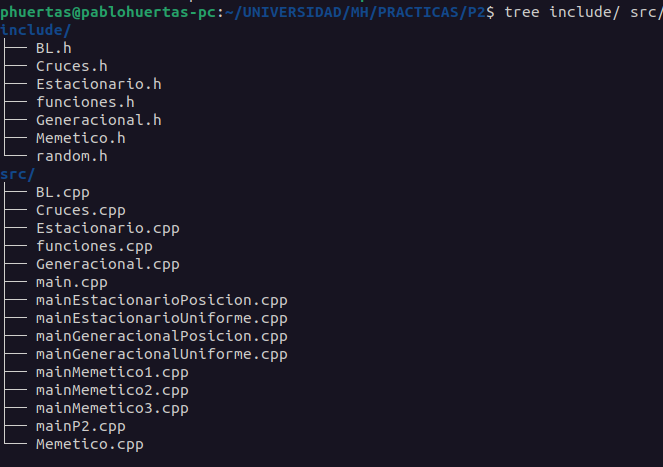
\includegraphics[scale=0.5]{TreeIncludeSrc.png}
    \caption{Diagrama en forma de árbol de los ficheros utilizados}
\end{figure}

\vspace{10mm}
El fichero makefile contiene las ordenes necesarias para compilar el proyecto, 
que básicamente lo que hace es compilar el fichero \emph{main.cpp} y generar el ejecutable 
enlazandolo con los archivos objetos funciones.o y random.o, que tambien son compilados.
He seguido la idea del pseudocódigo que se proporciona en Prado, tanto del seminario como 
del guion de la practica.
La directiva de compilacion usada para optimizar el programa es la de \emph{g++ -O2}
\newline Para ejecutar entonces el programa basta con situarse en la carpeta donde se 
encuentran estos directorios y llamar a make.
Luego con realizar una redimension de entrada básica al ejecutable funciona correctamente
\newline Por ejemplo: bin/main > data/ficheroentrada.txt
\newline Basicamente, este es el procedimiento considerado a la hora de desarrollar esta 
práctica, apuntes de la asignatura, algunas dudas resueltas en clase y algo de búsqueda 
de información sobre la STL.

\newpage
\section {\large EXPERIMENTOS Y ANÁLISIS DE RESULTADOS}
En ambos algoritmos hemos usado el mismo vector de semillas, que en cada iteración 
que ejecuta el programa el algoritmo, se coge la posicion i-esima del vector de semillas.
\newline El vector semillas es (1,2,3,4,5)
Por lo tanto en la primera iteracion se define la semilla como Random::Seed(1), y asi 
sucesivamente.
\newline Para comparar los resultados entre los dos algoritmos implementados en esta práctica, he hecho 
una tabla donde se muestran, para cada algoritmo, el tiempo medio y la dispersion media conseguida entre 
las 5 iteraciones conseguido con cada uno de los ficheros de datos.

\vspace{10mm}
\begin{figure}[h]
  \centering
   \subfloat[Tabla de resultados de Greedy]{
     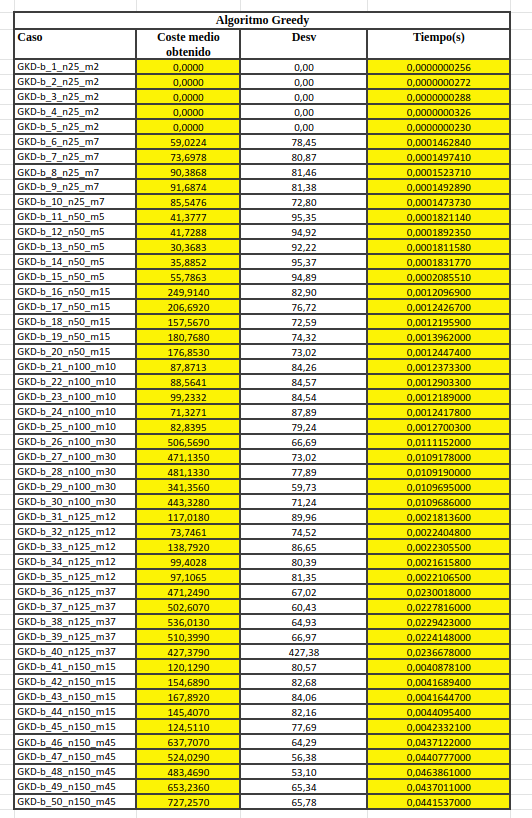
\includegraphics[width=0.3\textwidth]{TablaGreedy.png}}
   \subfloat[Tabla de resultados de BL]{
     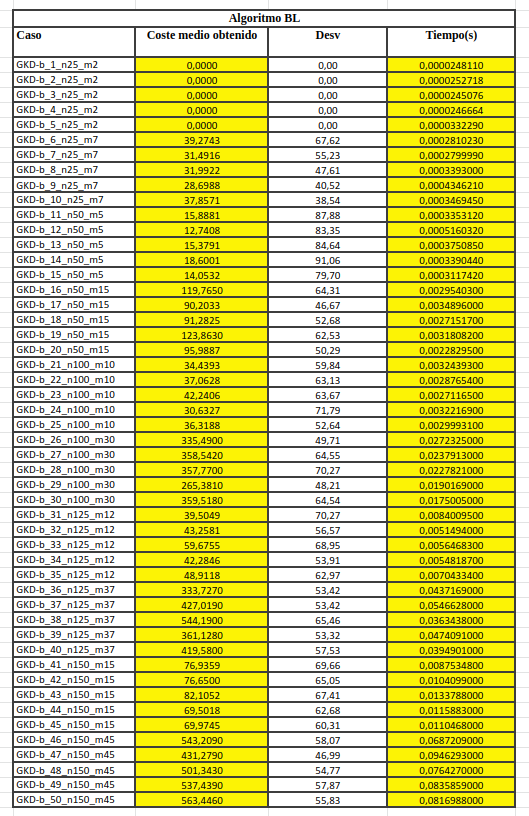
\includegraphics[width=0.3\textwidth]{TablaBL.png}}
  \caption{Tablas de resultados de Greedy y BL}
\end{figure}

\begin{figure}[h]
  \centering
   \subfloat[Desviacion y tiempo de Greedy]{
     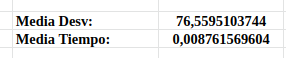
\includegraphics[width=0.3\textwidth]{DesvGreedy.png}}
   \subfloat[Desviacion y tiempo de BL]{
     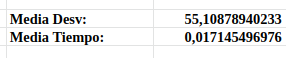
\includegraphics[width=0.3\textwidth]{DesvBL.png}}
  \caption{Desviaciones y tiempos de Greedy y BL}
\end{figure}

\vspace{10mm}
Observando los datos de las tablas, podemos observar que el algoritmo greedy tiene un 
tiempo menor que busqueda local, mientras que tiene una mayor desviacion, lo que quiere decir 
que sus resultados de dispersiones son peores.
\vspace{10mm}
\newline \textbf{¿Por qué Greedy tiene tiempos menores?}
\newline El algoritmo greedy es más eficiente respecto a lo que tiempo se refiere, 
ya que :
\begin{description}
  \item[Generacion de primera solucion]
  El algoritmo greedy solo tiene que generar dos elementos aleatorios a introducir 
  en la primera solucion, mientras que el algoritmo de busqueda local tiene que 
  generar aleatoriamente una solucion completa.
  \item[Generacion de vecindario]
  El algoritmo de Busqueda Local tiene que generar el vecindario completo, lo que requiere un 
  coste de O(X*Y), siendo X el numero de elementos de la solucion, e Y el número de elementos restantes.
  Ya que el conjunto de solucion junto a los restantes son los N elementos, este paso tiene un coste 
  de O(N), lo que supone una diferencia de tiempo con respecto a Greedy
  \item[Evaluacion de funcion objetivo]
  En este caso, los dos algoritmos se conforman de forma muy parecida, ya que se realiza 
  una factorización en el cálculo del Vector de Distancias en ambos, por lo que no se pueden 
  extraer conclusiones de aquí.
  \item[Actualización de la solucion constante]
  El algoritmo Greedy actualiza sí o sí la solución al final de cada iteracion, ya que 
  aunque ninguno mejore la dispersion, se escoge el que menos la empeore. Si el algorimo de 
  Busqueda Local no encuentra ningun vecino que mejore la dispersion, termina su ejecución.
\end{description}
Aunque estas diferencias no sean muy significativas, a la hora de evaluar muchas ejecuciones 
de estos algoritmos, encontramos como se acentúa más la diferencia.
\vspace{5mm}

\textbf{¿Por qué BL tiene menor media de Desviación?}
\newline El algoritmo de Busqueda Local tiene una menor media de desviacion que el algoritmo 
Greedy, es decir, que las dispersiones obtenidas de media con el algoritmo de Busqueda Local son 
menores(y por consiguiente, mejores) que las obtenidas por el algoritmo Greedy.
La desviacion se calcula como la media de las desviaciones, en porcentaje, del valor obtenido 
por cada metodo en cada instancia respecto al mejor valor conocido para ese caso.
\vspace{10mm}
\begin{equation}
  \textbf{Desviacion} = 
  100*\sum_{i=1}^n
  \frac{ValorAlgoritmo_i - MejorValor_i}{ValorAlgoritmo_i}
\end{equation}

\vspace{10mm}
Por lo tanto, tenemos unos datos de referencia, que contienen el mejor coste obtenido para 
cada instancia del problema.
El algoritmo de Busqueda Local obtiene mejores dispersiones de media que Greedy, y esto es gracias a que 
este algoritmo tiene mas probabilidad de encontrar mejores soluciones.
\newline Al generar el vecindario completo se asegura que si no se encuentran mejores 
dispersiones, no las selecciona, al contrario que Greedy, que aunque ninguno mejore la dispersion 
añade a la solucion el que menos la empeore.
\newline Esto evita que el algoritmo de Busqueda Local vaya hacia soluciones peores(mínimos locales), y siempre 
se asegure que cuando actualiza la solucion es para una mejor dispersion. 
\newpage En cambio, Greedy acepta soluciones peores a la actual, y esto puede hacer que caiga en mínimos locales,
y al siempre añadir elementos a la solucion, no poder salir de ellos.

\begin{figure}[h]
  \centering
  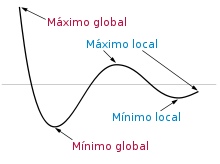
\includegraphics[scale=0.5]{MinLocal.png}
  \caption{Gráfica que muestra el comportamiento de una búsqueda de una solucion}
\end{figure}

\begin{figure}[t]
  \centering
  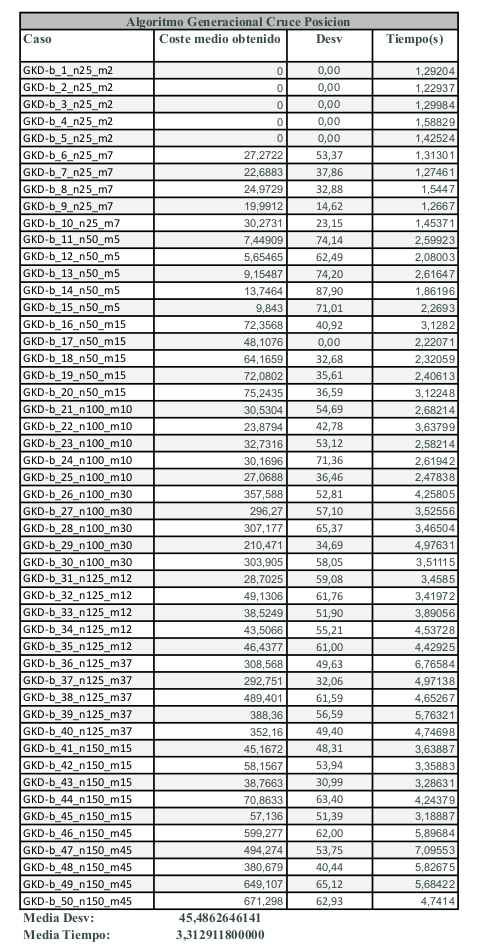
\includegraphics[width=0.75\textwidth]{capturastablas/AGG-Posicion.png}
  \caption{Desviaciones y tiempos de Algoritmo Genetico Generacional con Cruce \\
  Basado en Posicion}
\end{figure}

\begin{figure}[h]
  \centering
  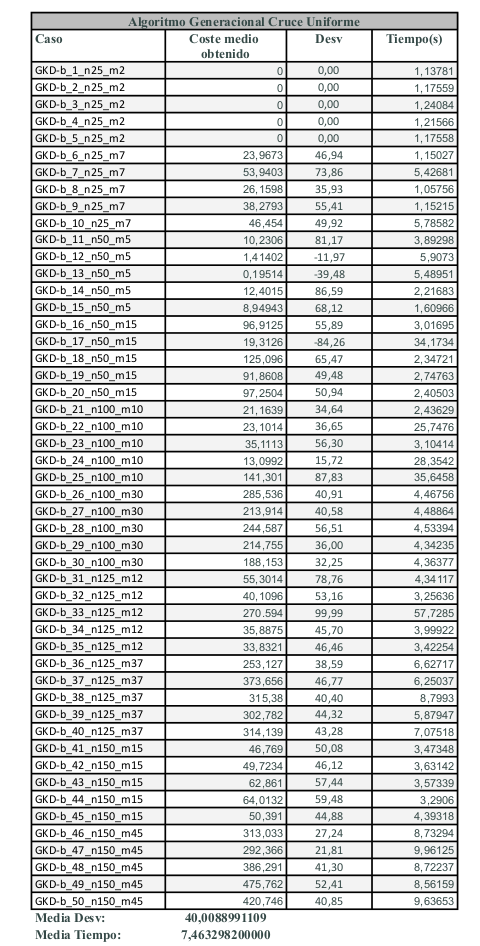
\includegraphics[width=0.75\textwidth]{capturastablas/AGG-Uniforme.png}
  \caption{Desviaciones y tiempos de Algoritmo Genetico Generacional con Cruce \\
  Uniforme}
\end{figure}

\begin{figure}[h]
  \centering
  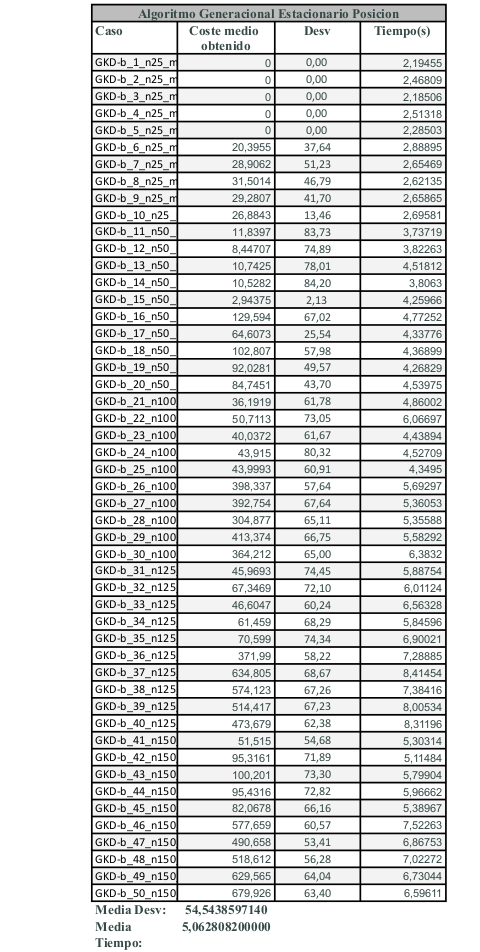
\includegraphics[width=0.75\textwidth]{capturastablas/AGE-Posicion.png}
  \caption{Desviaciones y tiempos de Algoritmo Genetico Estacionario con Cruce \\
  Basado en Posicion}
\end{figure}

\begin{figure}[h]
  \centering
  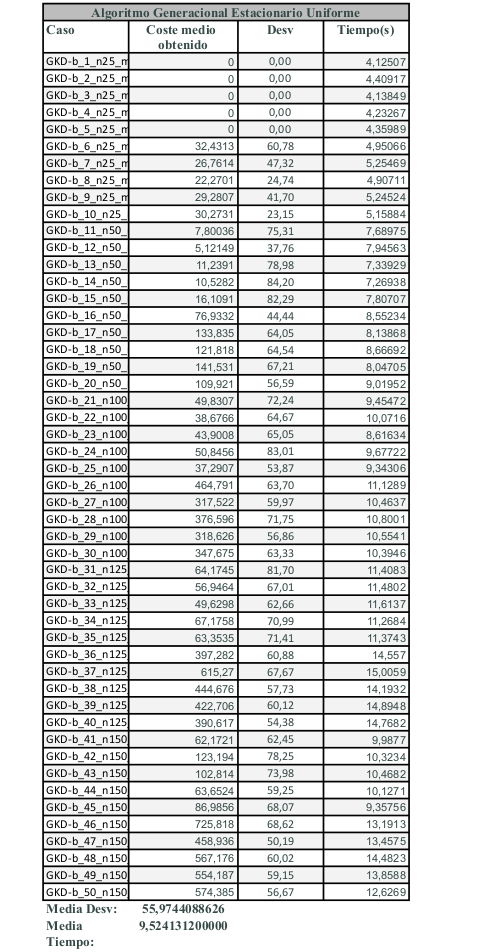
\includegraphics[width=0.75\textwidth]{capturastablas/AGE-Uniforme.png}
  \caption{Desviaciones y tiempos de Algoritmo Genetico Estacionario con Cruce \\
  Uniforme}
\end{figure}

\begin{figure}[h]
  \centering
  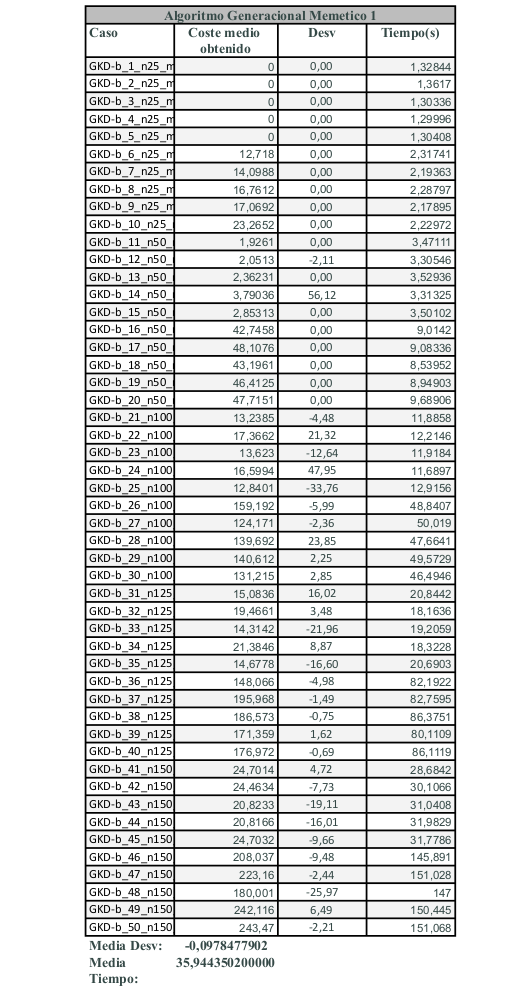
\includegraphics[width=0.75\textwidth]{capturastablas/Memetico1.png}
  \caption{Desviaciones y tiempos de Algoritmo Memetico \emph{AM-(10,1.0)}}
\end{figure}

\begin{figure}[h]
  \centering
  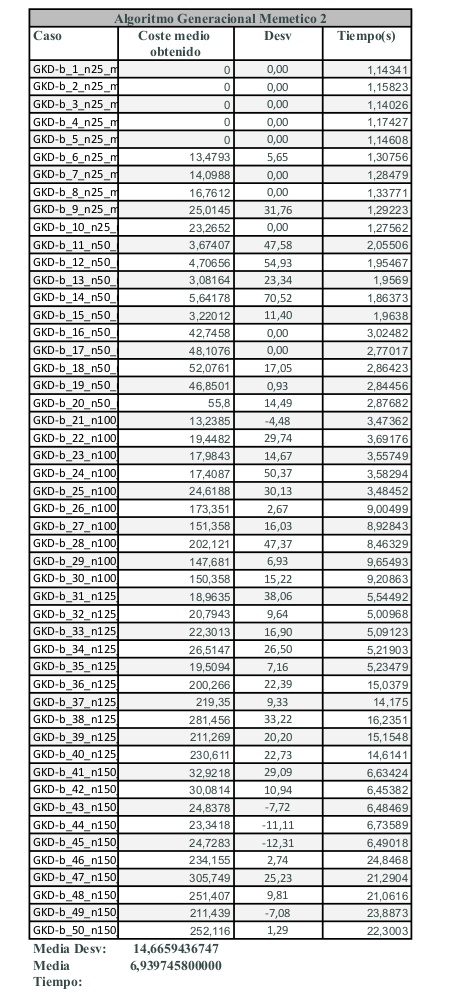
\includegraphics[width=0.75\textwidth]{capturastablas/Memetico2.png}
  \caption{Desviaciones y tiempos de Algoritmo Memetico \emph{AM-(10,0.1)}}
\end{figure}

\begin{figure}[h]
  \centering
  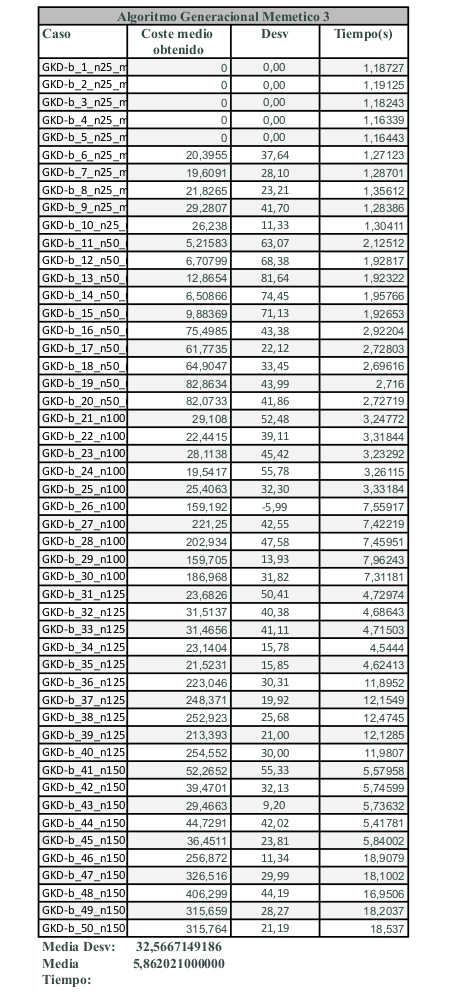
\includegraphics[width=0.75\textwidth]{capturastablas/Memetico3.png}
  \caption{Desviaciones y tiempos de Algoritmo Memetico \emph{AM-(10,0.1mej)}}
\end{figure}

\subsection{Tabla resumen}
\begin{table}[h]
  \begin{center}
    \begin{spacing}{1.5}
    \begin{tabular}{| l | l | l | }
      \hline
      \textbf{Algoritmo} & \textbf{Desviación media} & \textbf{Tiempo (en segundos)} \\ \hline
      \emph{Greedy} & 76,5595103744  & 0,008761569604 \\ \hline

      \emph{BL} & 55,10878940233 & 0,017145496976 \\ \hline

      \emph{AGG-Uniforme} & 40,0088991109 & 7,463298200000 \\ \hline

      \emph{AGG-Posición} & 45,4862646141 & 3,312911800000 \\ \hline

      \emph{AGE-Uniforme} & 55,9744088626 & 9,524131200000 \\ \hline

      \emph{AGE-Posición} & 54,5438597140 & 5,062808200000 \\ \hline

      \emph{AM-(10,1.0)} & -0,0978477902 & 35,944350200000 \\ \hline

      \emph{AM-(10,0.1)} & 14,6659436747 & 6,939745800000 \\ \hline

      \emph{AM-(10,0.1mej)} & 32,5667149186 & 5,862021000000 \\ \hline

    \end{tabular}
    \end{spacing}
    \caption{Tabla de medias de desviaciones y tiempos de los algoritmos}
  \end{center}
\end{table}

Observando la tabla, podemos ver que el algoritmo que mejores tiempo consigue 
es el memetico donde cada 10 iteraciones se realiza una busqueda local completa por cada 
cromosoma de la poblacion actual, es por eso que tiene los tiempos mas altos.
Esto tiene sentido ya que cada 10 iteraciones todas los cromosomas de la poblacion 
mejoran con dicho algoritmo, por lo que no va a quedarse estancado en optimos locales, escapando 
muy rapido de ellos.
\vspace{3mm}
\newline Vemos una mejora evidente en el algoritmo genetico de esquema generacional frente al 
del esquema estacionario, esto se debe a que el esquema estacionario no mejora con tanta rapidez
como lo hace el generacional, ya que como mucho en cada iteracion podra mejorar 2 soluciones, mientras que el 
generacional puede mejorar hasta n-1 soluciones, siendo n el numero de cromosomas de la poblacion, ya que es 
un algoritmo elitista, que nunca pierde la mejor solucion de la poblacion actual antes de ser 
reemplazada por la siguiente.
\vspace{3mm}
\newline Las diferencias entre el AGE-Uniforme y el AGE-Posición no son significativas por el fitness 
obtenido, pero si por el tiempo de ejecucion, ya que el operador de cruce basado en posicion 
requiere mucho menos tiempo que el uniforme. Esto se debe a que el uniforme en muchas ocasiones,
llama al operador de reparación, que tiene un coste bastante alto, y además solo se obtiene 
un hijo con los dos padres, mientras que en el basado en posicion, se obtienen 
dos hijos de dos padres lo que acelera bastante el proceso.
Estas diferencias son aplicables igualmente en el esquema generacional, aunque la probabilidad
de cruce sea 0.7 en vez de 1
\vspace{3mm}
\newline Respecto a los algoritmos memeticos, el algoritmo ganador respecto a fitness como he 
comentado anteriormente es el de la primera variante, ya que al aplicar una busqueda local sobre todos 
los cromosomas, nunca se queda estancado en la mejora de soluciones.
El de la segunda variante, que aplica la busqueda local sobre un 10\% aleatorio de los cromosomas 
de la poblaicon, es el segundo mejor que hemos conseguido respecto a fitness, pero es un poco peor respecto 
a tiempo que la ultima variante. Este buen fitness conseguido se debe a la aleatoriedad de los cromosomas
seleccionados para la busqueda local, ya que los cromosomas que se seleccionan aleatoriamente 
pueden estar en maximos locales, por lo que gracias a la busqueda local, se pueden mejorar dichas 
soluciones.
\vspace{3mm}
\newline El ultimo como vemos obtiene el peor resultado respecto a fitness de los 3 algoritmos memeticos, y esto se debe a que al 
aplicarse la busqueda local sobre el 10\% de mejores soluciones, muchas veces la búsqueda local 
se queda estancada en dichas soluciones porque en el entorno no se encuentra mejora, entonces al aplicarse esa 
busqueda sobre las mejores no se mejora tanto como la anterior variante, que aleatoriamente es probable 
que cada x iteraciones seleccione cromosomas que se encuentran estancados, mientras que esta 
variante no, siempre va a coger a los mejores y por el elitismo del esquema generacional, es probable que 
se aplica muchas veces a los mismos cromosomas.


\end{document}